\section{Methodology}
\label{sec:methodology}

The experiment separated two roles. Humans designed the measuring apparatus and
fixed the rule by which pipeline code was admitted or removed. The agent
designed and implemented every step of the pipeline that turned a question into
SQL. The agent analyzed the run traces. Humans could inspect a selected group
of questions in detail before a full development run.

\begin{figure}[t]
  \centering
  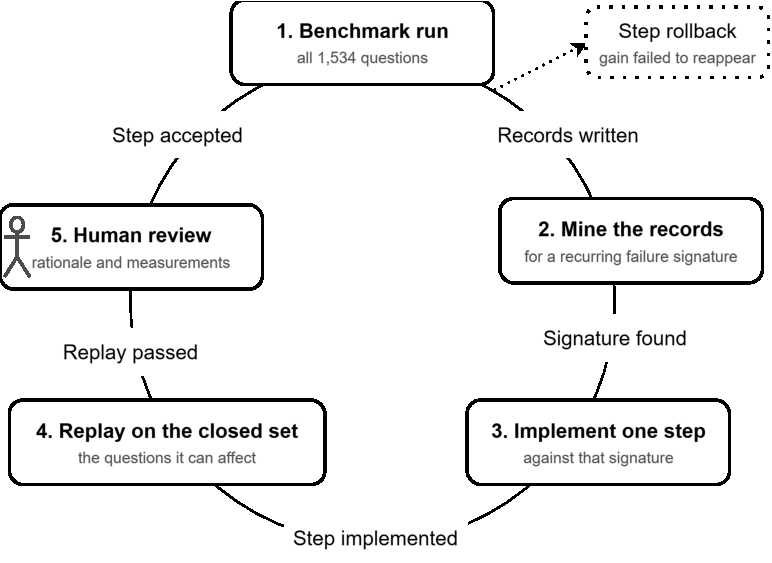
\includegraphics[width=\columnwidth]{harness_iccq-fig}
  \caption{The harness and the development cycle inside it. A full benchmark
  run leaves records; the agent mines them for a recurring failure signature,
  implements one step against it, and replays the change over the closed set
  of questions it can affect. Human review admits the step into the next
  pipeline version, whose full run measures the combined effect, and a later
  run that argues against a step removes it.}
  \label{fig:harness}
\end{figure}

\paragraph{The harness.} A single command ran a named pipeline version over a
question set and produced the entire record of that run
(Figure~\ref{fig:harness}). On disk, a timestamped
directory held the fully resolved configuration, pinning the pipeline version,
the models, and the question subset. Beside it grew an append-only predictions
file with one record per question, carrying the question and its evidence hint,
the reference and generated SQL, the rows each of them returned, and the
verdict. A run log and a diff report over every miss completed the directory.
The same execution was mirrored as a telemetry stream into a local Arize
Phoenix instance,\footnote{\url{https://docs.arize.com/phoenix}} one span per
step recording its kind, its duration, what it
saw and what it decided, and, for model calls, the prompt, the response, and
the tokens they cost. Every run registered itself as an experiment against a
question set pinned as a dataset, so any two runs could be aligned question by
question.

\paragraph{Scoring.} The harness judged an answer by running it. It executed
both the generated query and the reference query against the database and
compared the two sets of result rows as unordered sets, the local execution-accuracy measure used for accept-or-revert decisions. Scoring in this form is dynamic analysis
over the generated artifact: nothing is inferred from how a query reads, and
the verdict comes from what it returns on a real database.

\paragraph{Classifying disagreements.} A wrong answer was decomposed rather
than counted. For each question the predictions file named the rows missing
from the generated result and the rows that should not have been there. The
diff report paired reference and generated rows side by side and sorted each
mismatching value into one of three kinds: the same number written in a
different format, two date-like values, or genuinely different
values. A miss therefore stated in what way it was wrong, in text that could be
grepped and clustered across a run.

\paragraph{Step self-reporting.} Every step reported on itself. The runner
contributed only the step's kind and its timing to the span, while the account
of what the step received and what it decided came from the step's own code and
was written to the run log as well. Adding a step meant following that
convention, so the agent's own additions arrived instrumented, and the next run
already showed how often a new step fired, on what evidence, and what it
changed. Clustering those records over a run is what localized a defect,
tracing a signature that recurred across many questions to the step that
produced it or should have caught it. Such localization is statistical over a
corpus rather than exact over one failing execution---a weaker instrument than
a failing test and a much stronger one than an aggregate score.

\paragraph{The documented interface.} One instruction file in the agent's
working environment described the mechanics: the command that started a run,
the artifacts it left and where they lived, how to query the telemetry store,
and how to add a step. The file covered measurement discipline and nothing
else. It named no text-to-SQL technique, diagnosed no failure, and proposed no
step.

\paragraph{The development cycle.} The agent was Claude Opus, versions 4.6
through 4.8 as they became available over the course of the project, working
in Claude Code.
One turn of the loop (Figure~\ref{fig:harness}) began with a full run over the
development set. The agent
read its records until a failure signature recurred across enough questions to
warrant code, then implemented one step aimed at that signature, with
self-reporting included, and replayed the modified pipeline over the closed set
of questions the change could affect: the failures that motivated it, together
with the passing questions it could plausibly break. A step that repaired its
targets and left its neighbors intact was bundled with the other accepted
changes into the next named pipeline version, and that version ran over all
1,534 development questions. Comparing the two versions question by question
reported how many answers had been gained and how many lost.

Before a full run, proposals were screened for a target group of at least
ten questions, to avoid spending tokens on changes with too little expected
reach; this was not a requirement of ten net corrections after execution.

\paragraph{Human review and rollback.} Humans reviewed the rationale of each
proposed step together with the measurements attached to it, and wrote none of
the pipeline code. Acceptance was provisional. At least seven changes cleared review and
their replay test only to be removed later, when the gains that had justified
them failed to reappear in subsequent full runs. In the clearest case a cluster
of challenging misses shared one cause---a reference query routing through a
bridge table the generated query never joined. The step the agent wrote against
it closed foreign-key paths across bridge tables and ran in three full
benchmark runs. The same questions stayed wrong in all three, and the step was
removed.

\paragraph{The gate.} Stated as a procedure, admission imposed four
requirements. A
change had to originate in a defect signature already localized in the records
of a completed run, not in a hypothesis about the task. It had to be measured
first over the closed set of questions it could touch, where its repairs and
its collateral damage were visible at once. It then had to be re-measured over
the full question set inside a named pipeline version, competing there with
everything else that version carried. And it stayed removable, so a later run
arguing against a step took the step out regardless of the measurement that had
first admitted it. Nothing else counted: neither the plausibility of a
rationale nor a reviewer's opinion of the code could admit a step on its own.
